% #############################################################################
% This is Chapter 3
% !TEX root = ../main.tex
% #############################################################################
% Change the Name of the Chapter i the following line
\fancychapter{PM10 Monitoring, Interpolation and Visualization System}
\cleardoublepage
% The following line allows to ref this chapter
\label{chap:architecture}

%Reviewed literature has shown the current state of information available regarding urban air quality. The same can be said for the state of \ac{LPWAN} technology evolution and the current available and most used interpolation algorithms applied in the field of air quality spatial modelling. 

The methodologies and implementation details concerning the systems developed in this work are presented and explained in this section.

First, a small system that measures PM10 and retrieves them through NB-IoT to a server, which saves them in a database, was developed. This system consists of an NB-IoT module for communication and a PM low-cost sensor. Its performance was compared with one of the official standard PM sensors used by \ac{APA} in standard monitoring stations in Lisbon.

Second, SIMs were tested and assessed with the use of data from QualAr, from 2013 to 2017, with a focus on its comparison against FBNs, which have been shown to be promising when interpolating with sparse datasets \cite{Tome2014}.

Finally, a web application for the presentation of live high-resolution PM pollution rates was built, within a similar area to the city of Lisbon, covering the stations that provide data for the interpolations.

% #############################################################################
\section{Low Cost NB-IoT PM10 Monitoring System} 

The NB-IoT PM10 monitoring system was developed to evaluate how well these type of equipment could integrate current standard air monitoring networks, expanding its size, and consequently providing better data for spatial modelling approaches.

A low cost sensor was used to measure PM10 concentration in the air at a constant rate with relatively low power consumption. Sensor outputs were retrieved and processed by a programmable micro-controller.

The main requirements of this system were low production costs, a \ac{SFF}, low power consumption as well as long range transmission. A low bit rate is acceptable, since the measurement rate is also relatively low. The processing power required is low, since a low amount of data is processed by the micro-controller.

\subsection{Development and Composition}

NB-IoT was the LPWAN techology used in this work, due to the agreements between INESC-ID and Altice Portugal and NOS for its usage for research purposes, and considering the technology characteristics presented in \Cref{chap:back}.

\begin{itemize}[leftmargin=0.0mm]
  \item[] \textbf{SODAQ SARA SFF R412M}
\end{itemize}

\noindent
The development board used in this work is the SODAQ SARA SFF R412M board, which is an industry standard IoT developer board, with low power consumption, which allows the use of both NB-IoT and LTE-M networks, implying coverage across Europe, North America, Africa and Asia, with 62.5 kbit/s upload and 27.2 kbit/s download rates, and Over-The Air firmware updates \cite{U-blox}. This board contains an integrated micro-controller, the Atmel SAMD21, which allows it to be programmed through the same tools as every Arduino compatible board.

Subscriber identity module cards provided by the mobile operators NOS and Altice Portugal were used for this board remote communications with NB-IoT. These card were previously configured by the mobile operators according to the specifications needed for its optimal use in NB-IoT devices.

AT commands are used to communicate through the NB-IoT module. 
The commands used in the implementation of the developed system, and in the micro-controller program, along with its purpose are presented in \Cref{table:atCommands}. These are available in the SODAQ AT command manual \cite{U-Blox2018}.

\renewcommand\arraystretch{1.5}
\begin{table}[ht]
\centering
\caption{AT commands used with the NB-IoT micro-controller.}
\label{table:atCommands}
\begin{tabular}{l l} % centered columns (4 columns)
\toprule
Command&Functionality\\
\midrule
AT+CFUN&Sets the mobile terminal to full functionality\\
AT+CGATT&GPRS Attach\\
AT+USOCR&Create a socket\\
AT+USOST&Writes the specified amount of data to the remote address\\
AT+USOCL&Close socket\\
\bottomrule
\end{tabular}
\end{table}

The code developed for the micro-controller was written in the Arduino IDE environment, and consists of an internal loop that is continuously receiving measures from the sensor, and every 15 minutes, it makes the averages of the measures taken in that period and sends it through the NB-IoT AT commands, if there is network coverage.

The server code that receives the data from the NB-IoT modules is written in Python. In this program, an \ac{UDP} socket is used to receive packets from the sensor nodes. These contain the sensor location, id, a PM10 and a PM2.5 value, corresponding to the respective 15 minute averages. After receiving the data, it is stored in a database directly from the server.


\begin{itemize}[leftmargin=0.0mm]
  \item[] \textbf{Plantower PMS5003}
\end{itemize}

\noindent
A sensor from Plantower was used for the measurement of PM concentration, specifically the PMS5003, a low-cost light-scattering optical sensor with a built-in fan that provides air circulation, widely used and reviewed in the literature \cite{Kuula2019}\cite{Zheng2018}\cite{Zheng2019}\cite{Wendt2019}\cite{Ford2019}\cite{Manikonda2016}\cite{Liu2017}\cite{Sayahi2018}. This sensor measures both PM10 and PM2.5 concentration in suspended particles in the air, and outputs it through a digital signal, processed by a microprocessor, in real-time. Its minimum distinguishable particle diameter is 0.3 micrometers. Since it provides a low cost and low consumption profile, with an SFF, and also compatibility with Arduino boards, this sensor is optimal for this use case.


%A more detailed description of this sensor can be found in \cite{Yong2016}.

Its power supply requirements are 5V DC, and a maximum of 100mA. It can withstand operating temperatures from -10ºC to 60ºC, as well as relative humidity from 0 to 99\%. It is documented by the manufacturer that its maximum consistency error is of 10 μg/m³ if the measured values range from 0 to 100 μg/m³, and of 10\% from 100 to 500 μg/m³.

The PM sensor has two modes of functioning, the active and the passive mode. In the active mode, the sensor is always working and constantly sending digital data to the micro-controller. The data transport protocol works by sending 32 bytes periodically, of which each byte represents a different value. The first four and last four bytes are used for error checking. Bytes from 5 to 10 represent the PM concentration of suspended particles with the maximum diameter of 1, 2.5 and 10 respectively, for factory environments. Bytes from 11 to 16 have the same meaning, but in this is case for atmospheric environments. Finally, remaining bytes represent the number of particles with diameter beyond a certain value, which is a metric that is not in the scope of this thesis. This mode is depicted in \Cref{table:active-mode}.
In this work, only the bytes from 11 to 16 are of interest.

\renewcommand\arraystretch{1.5}
\begin{table}[ht]
\centering
\caption{Bytes in PMS5003 Active Mode functionality.}
\label{table:active-mode}
\begin{tabular}[t]{l>{\raggedright\arraybackslash}p{0.815\linewidth}}
\toprule
Byte Interval&Functionality\\
\midrule
1 to 4&Error check\\
5 to 10&PM10, PM2.5 and PM1.0 concentration under factory environment\\
11 to 16& PM10, PM2.5 and PM1.0 concentration under atmospheric environment\\
16 to 28&Number of
particles with diameter beyond 10, 5, 2.5, 1, 0.5 and 0.3 μm in 0.1 liters of air.\\
29 to 32&Error check\\
\bottomrule
\end{tabular}
\end{table}%


The passive mode is an host transport protocol, in which the micro-controller makes requests to the sensor and it replies accordingly. Due to the requirements on the sensor end, the active mode was the mode used in this work.


\begin{itemize}[leftmargin=0.0mm]
  \item[] \textbf{Step Up Voltage Converter}
\end{itemize}

\noindent
For the assembling of the SODAQ SFF R412M board with the PMS5003 sensor, a step up voltage converter is needed, since PMS5003 internal fan requires 5V DC power supply, and the SODAQ board can only output 3.3V. Despite this, the sensor high level of data pins is 3.3V. Therefore, the first iteration of this system can be presented as the one in \Cref{fig:ieec5}.


\begin{figure}[ht]
\centering
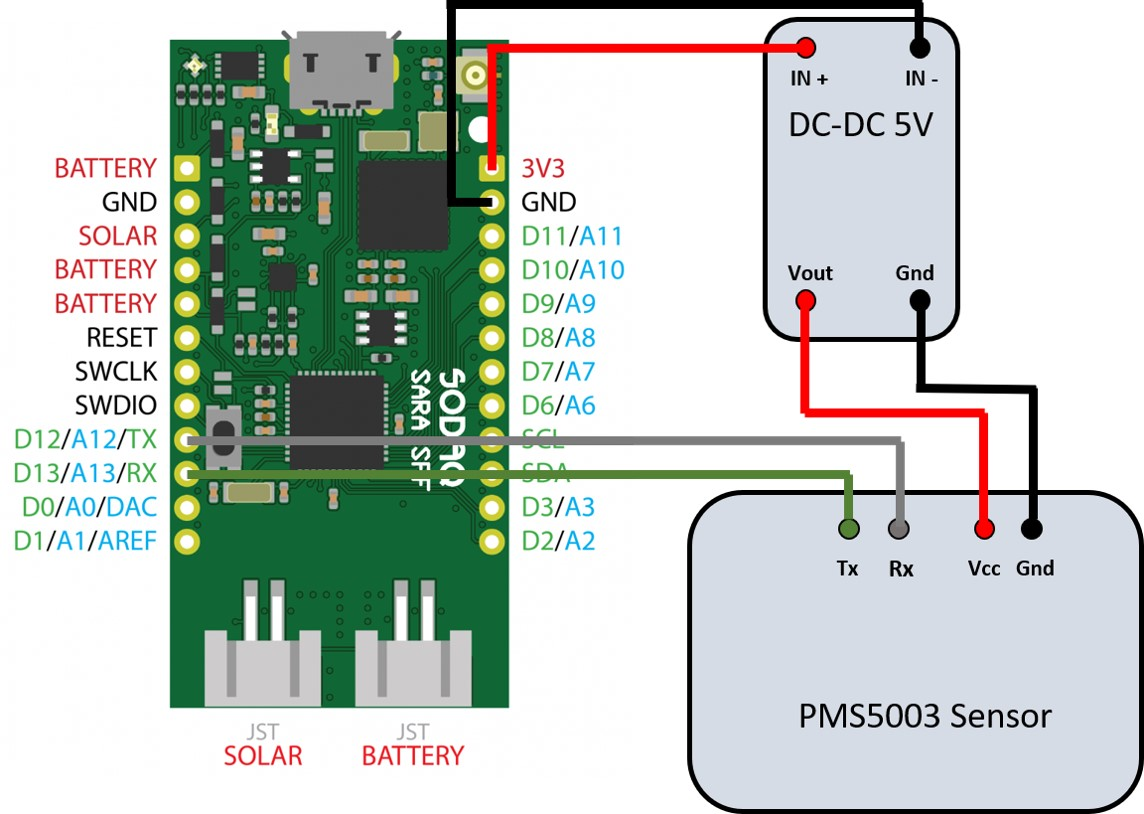
\includegraphics[width=0.6\textwidth]{./Images/ieec5.jpg}
\caption{First prototype of the developed PM monitoring system.}
\label{fig:ieec5}
\end{figure}

Similar to the behavior of the official monitoring networks, once data is collected from the sensors, 15 minute averages are calculated and sent to a server, which stores them in a database.

The developed system workflow is depicted in \Cref{fig:flowchart_monitoring_system}.

\begin{figure}[ht]
\centering
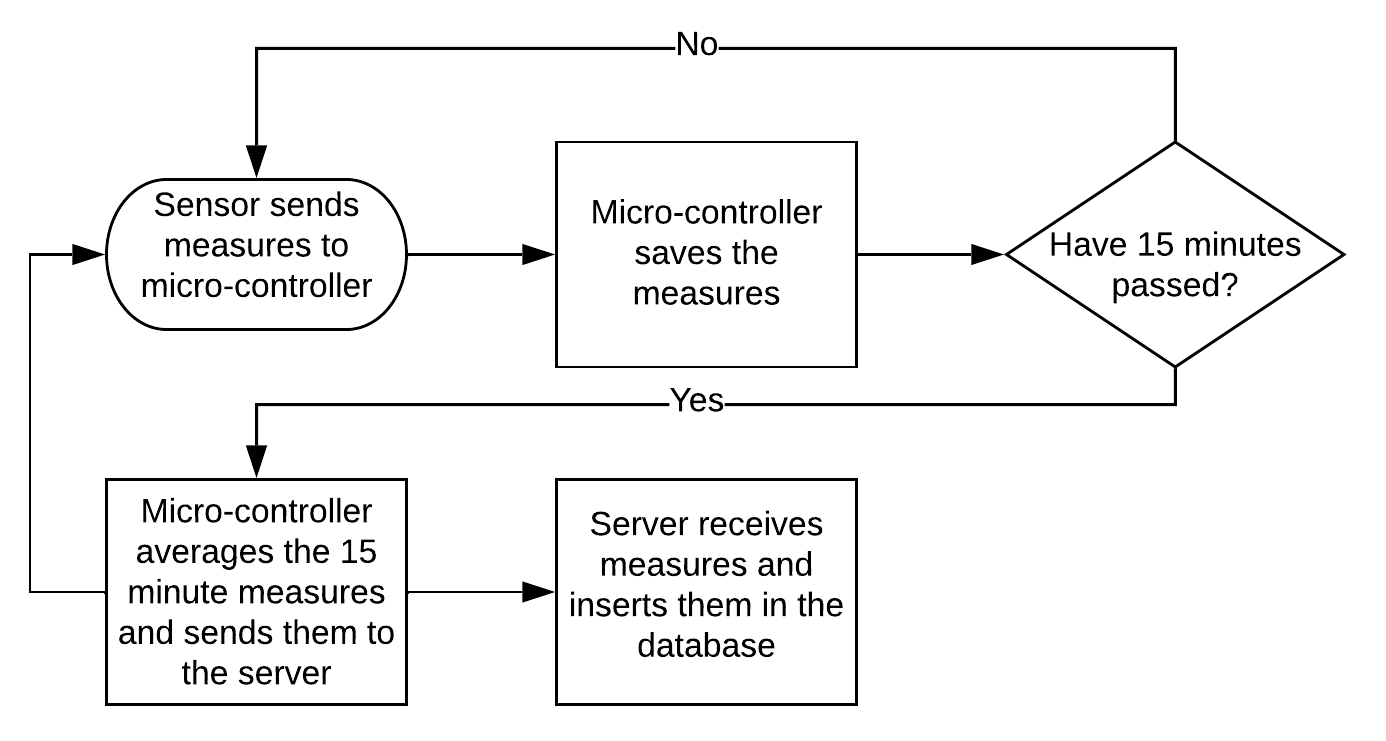
\includegraphics[width=0.75\textwidth]{./Images/flowchart_monitoring_system.png}
\caption{Overview of the developed monitoring system.}
\label{fig:flowchart_monitoring_system}
\end{figure}

\subsection{Placement and Behavior Analysis}

Both \ac{ENC} and the \ac{AVL} monitoring stations were used for the placement of the developed sensors.

Reference PM monitors are placed inside a container, and in order for air to reach the monitors, several teflon pipes are placed outside, within 2 meters of relative altitude, and the air is sucked through these pipes into the monitor container.

Similar behavior was intended to be replicated with the developed system with the junction of a vacuum pump and a plastic pipe to the developed system. However, to have better network coverage, the developed sensor had to be placed outside, in the top of the monitoring stations, next to the air entrance of the station and without any pipe, in a small box resistant to weather conditions and with an index of protection of 65. In \Cref{fig:circuit-final}, the final assembly of this system is presented.

\begin{figure}[ht]
\centering
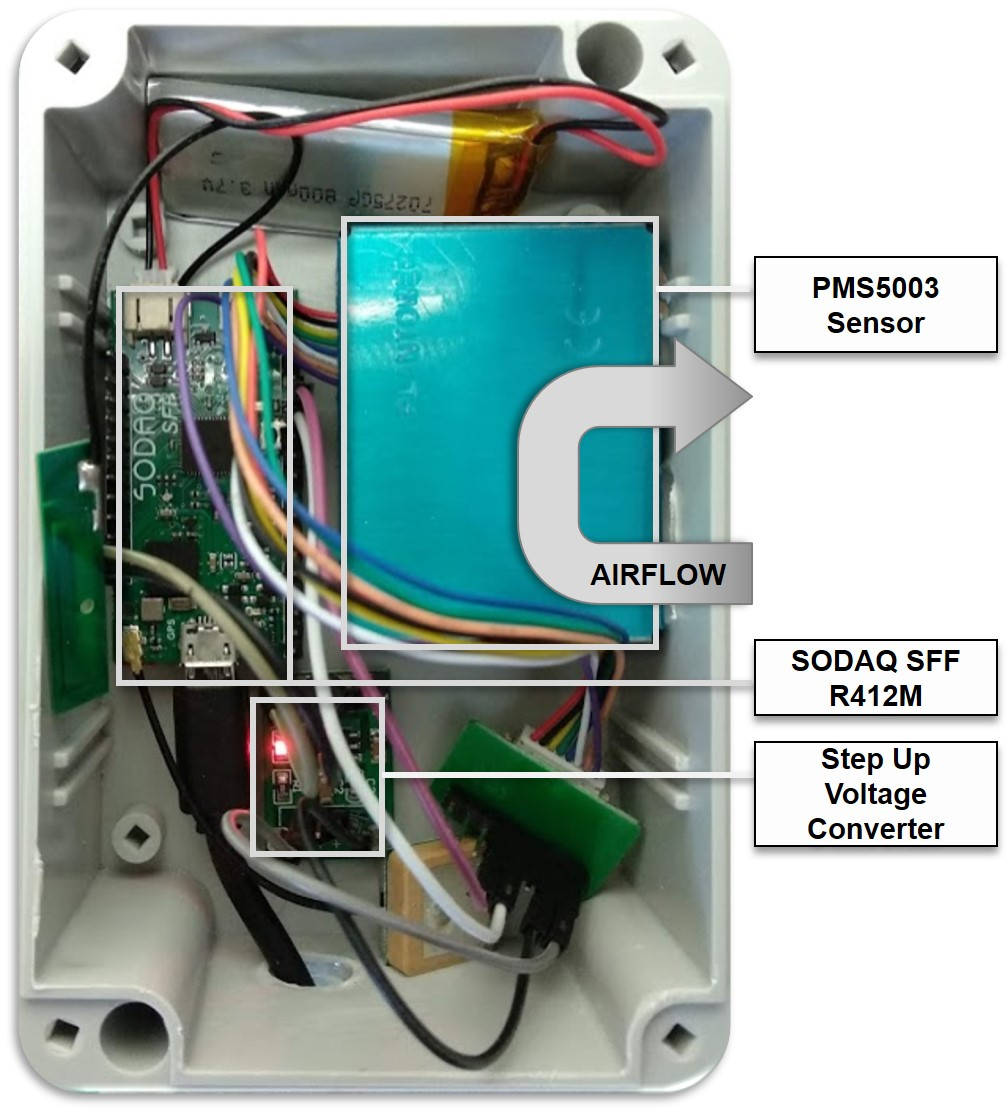
\includegraphics[width=0.45\textwidth]{./Images/circuit-final.jpg}
\caption{Final assembly of the developed monitoring system.}
\label{fig:circuit-final}
\end{figure}

%Aqui falta explicar que método será usado para fazer a calibração do sensor e talvez referênciar artigos onde esta técnica tenha já sido usada.
The developed system was placed during two weeks of July in AVL station, four weeks of August and two of September in ENC station and, finally, during the two final weeks of September in AVL station.

%\subsection{Functionality with SIMs}

%After the calibration process, based on the performance of the developed system in comparison to reference monitors, two main points can be made about it:

%\begin{enumerate}

%\item How low cost \ac{PM} monitors can be inserted in reference station networks in order to complement the data available to \ac{SIM}s, and also to help its assessment.

%The insertion of these type of systems in the current monitoring networks would greatly improve the spatial resolution of the data available for interpolation algorithms, which is crucial since the main obstacle in air quality spatial modelling is the low availability of data, as well as its sparsity.

%\item How low cost \ac{PM} monitoring systems perform against reference monitors with much higher purchase and maintenance costs.

%\end{enumerate}


% #############################################################################
\section{Spatial Interpolation Algorithms}

The main algorithms which are assessed in this work are FBN, OK and IDW. Additionally, simpler interpolation algorithms such as LI and NN are also tested. Data from 2005 to 2017 was extracted and analysed from QualAr website for the algorithms assessment. This data only concerns monitoring stations in the greater area of Lisbon,which corresponds to the area where air quality monitoring stations have the most spatial density in Portugal.

In this section, there is an overview of the data selection process, the algorithms parametrization and the tests that were done to assess the algorithms.

% Adicionar aqui informação se for possível fazer testes com algoritmos que levem em conta o tráfeog ou os ventos dominantes

\subsection{Dataset Selection}

In the greater area of Lisbon there is an air quality monitoring network composed of 14 monitoring stations, maintained by \ac{CCDR-LVT} \cite{QualAr}. Only 13 of these have operating PM10 sensors, from which only 10 are fully operating at the time of this work. Only 4 out of these have operating PM2.5 sensors. 

PM2.5 data was not regarded due to the lack of stations in the area of analysis. 

Only data from 2013 to 2017 was gathered since it is the most consistent overall, with measures from the considered stations, at high percentages of completeness (\Cref{table:completeness}).

From the five years of measures, a dataset of 43 506 hourly averaged measures was collected for each Lisbon PM10 measuring station. However, there were still many periods with incomplete data from some of the stations, since these were not working during certain periods. In order to remove data inconsistencies, the dataset was filtered based on the number of data per time interval. Each set was required to have at least 10 measures from all the considered stations, and at least 3 measures from the stations in the center of the network, presented in red in \Cref{fig:lx-stations-points}.

\begin{figure}[h]
\centering
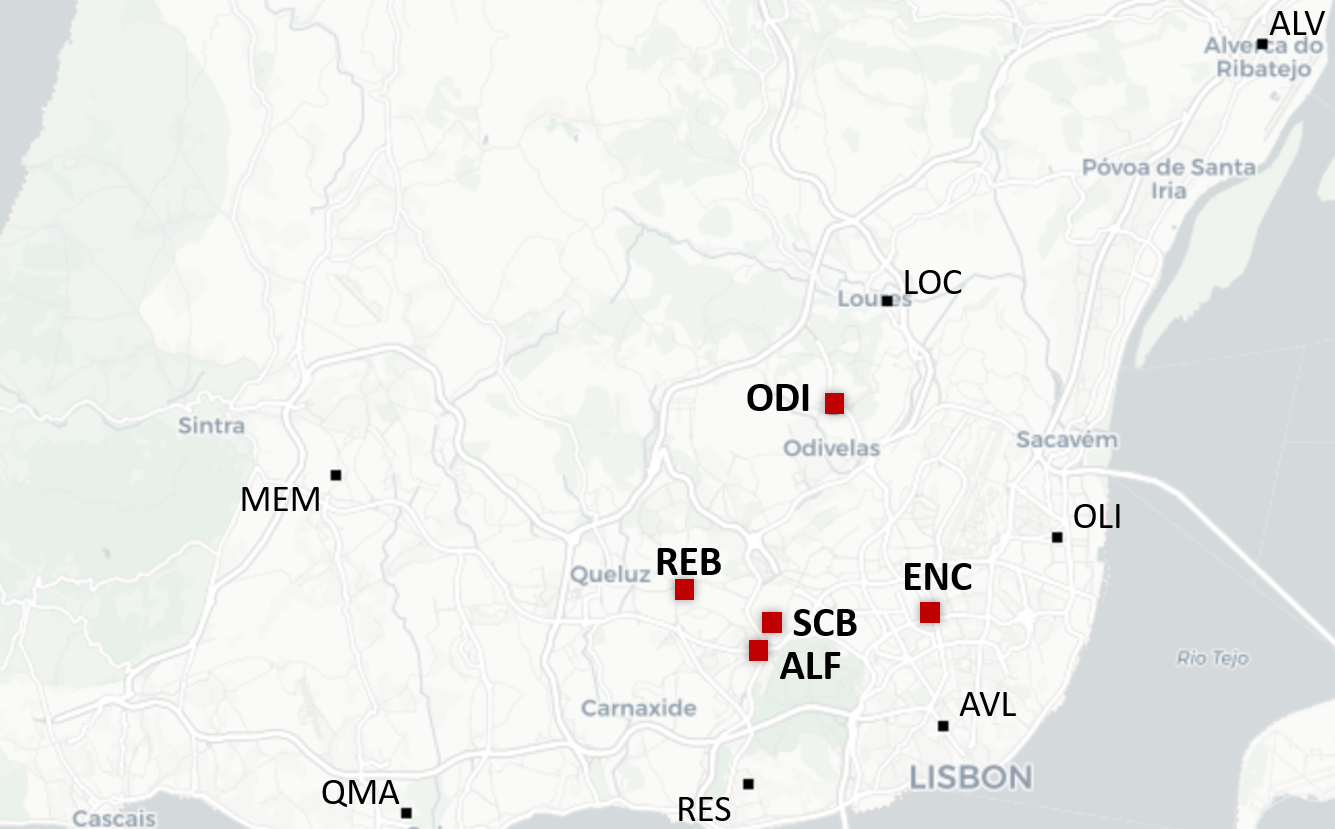
\includegraphics[width=0.7\textwidth]{./Images/lx-stations-points.png}
\caption{Considered stations in the greater area of Lisbon.}
\label{fig:lx-stations-points}
\end{figure}

In \Cref{table:completeness}, the percentages of completeness of each station before and after dataset filtering are presented. An increase of data completeness is evident in all stations. The \ac{ALF} station demonstrated very low completeness overall, before and after filtering, therefore it was removed from the dataset.

\renewcommand{\tabcolsep}{3pt}
\renewcommand\arraystretch{1.1}
\begin{table}[ht]
\centering
\caption{PM10 data completeness of considered stations before and after data filtering.}
\label{table:completeness}
\begin{tabular}{p{0.22\textwidth}>{\centering}p{0.08\textwidth}>{\raggedright}p{0.15\textwidth}>{\centering}p{0.15\textwidth}>{\centering}p{0.15\textwidth}>{\centering\arraybackslash}p{0.1\textwidth}}
\toprule
\multirow{2}{*}{Station}&\multirow{2}{*}{ID}&\multirow{2}{*}{Station Type}&\multirow{2}{*}{Area Type}&\multicolumn{2}{c}{Data Completeness (\%)}\\\cline{5-6}
&&&&Overall&Filtered\\
\midrule
Alfragide/Amadora&ALF&Background&Urban&1.40&2.85\\
Alverca&ALV&Background&Urban&97.47&99.96\\
Avenida da Liberdade&AVL&Traffic&Urban&96.49&99.21\\
Entrecampos&ENC&Traffic&Urban&76.40&99.50\\
Loures-Centro&LOC&Background&Urban&85.88&91.46\\
Mem Martins&MEM&Background&Urban&88.31&99.72\\
Odivelas-Ramada&ODI&Traffic&Urban&82.89&98.88\\
Olivais&OLI&Background&Urban&93.74&99.54\\
Quinta do Marquês&QMA&Background&Urban&89.30&99.55\\
Reboleira&REB&Background&Urban&68.88&96.88\\
Restelo&RES&Background&Urban&29.66&40.81\\
Santa Cruz de Benfica&SCB&Traffic&Urban&48.67&82.00\\
\bottomrule
\end{tabular}
\end{table}%

The \ac{ALV} station was also removed from the dataset, because it is located too far from the center stations, which would increase the problem sparsity and possibly degrade the algorithm performance. This data exclusion process can be observed in \Cref{fig:dataset-filtering}, where \textit{N} represents the size of each dataset.

\begin{figure}[ht]
\centering
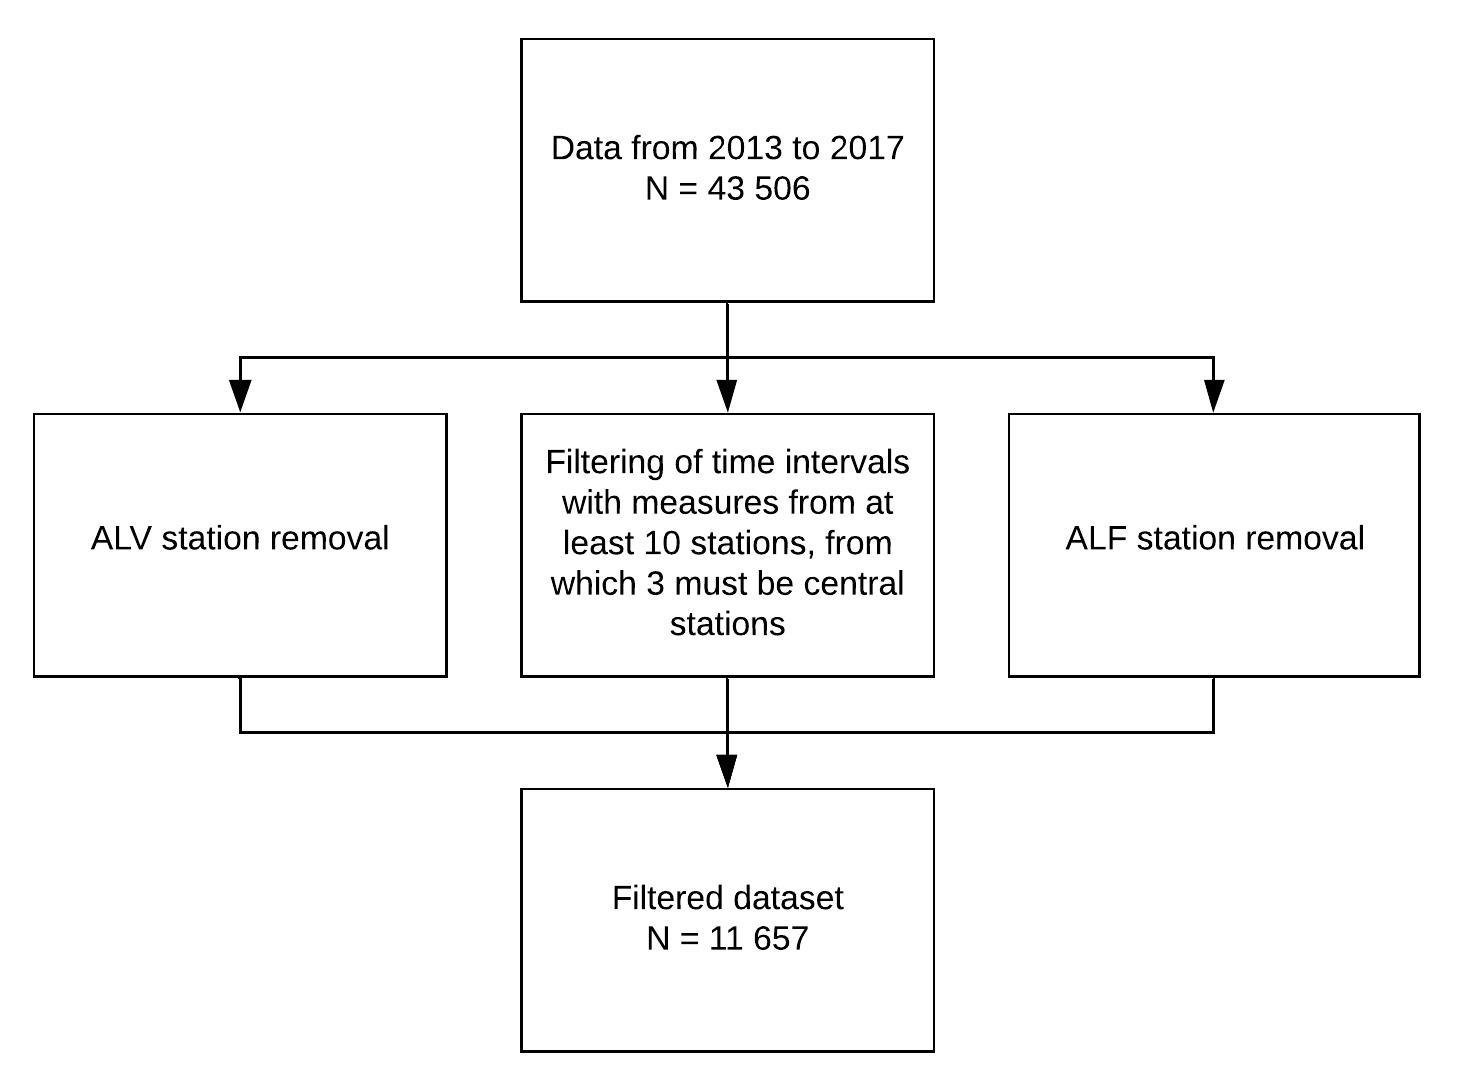
\includegraphics[width=0.8\textwidth]{./Images/dataset-filtering.jpeg}
\caption{Dataset exclusion process.}
\label{fig:dataset-filtering}
\end{figure}

The number of sets of measures in the dataset decreased from 43 506 measures in the initial dataset, to 11 657 in the filtered one. A map with the remaining Lisbon monitoring stations, after dataset filtering, is presented in \Cref{fig:map-filtered}. 

Data correlation was also calculated between every station and the center target stations. These coefficients help to explain the quality of the spatial prediction obtained by the various models. In \Cref{table:correlation-coef} these are presented, with an highlight of the stations which share higher linear correlation.

%\renewcommand{\tabcolsep}{3pt}
\renewcommand\arraystretch{1}
\begin{table}[h]
\centering
\caption{Correlation coefficient between target and remaining stations in the Lisbon monitoring network.}
\label{table:correlation-coef}
\begin{tabular}[t]{l>{\centering}p{0.1\linewidth}>{\centering}p{0.1\linewidth}>{\centering}p{0.1\linewidth}>{\centering\arraybackslash}p{0.1\linewidth}}
\toprule
&ENC&ODI&REB&SCB\\
\midrule
%ALF&1&0.53&0.47&0.42&0.54\\
%ALV&0.76&0.78&0.79&0.69\\
AVL&0.83&0.77&0.78&0.76\\
ENC&1&0.84&0.82&\textbf{0.81}\\
LOC&0.77&0.79&0.79&0.69\\
MEM&0.77&0.78&0.8&0.66\\
ODI&\textbf{0.84}&1&\textbf{0.86}&0.78\\
OLI&0.83&0.76&0.78&0.74\\
QMA&0.77&0.78&0.83&0.71\\
REB&0.82&\textbf{0.86}&1&0.8\\
RES&0.76&0.83&0.81&0.73\\
SCB&0.81&0.78&0.8&1\\
\bottomrule
\end{tabular}
\end{table}%

These were calculated with the Pearson correlation coefficient, which has been used in similar applications \cite{Deligiorgi2011}, and represents the linear correlation between two variables. 
The possible result values vary from 1 to -1, where 1 represents total positive linear correlation, 0 represents no linear correlation, and -1 total negative linear correlation.

\begin{figure}[ht]
\centering
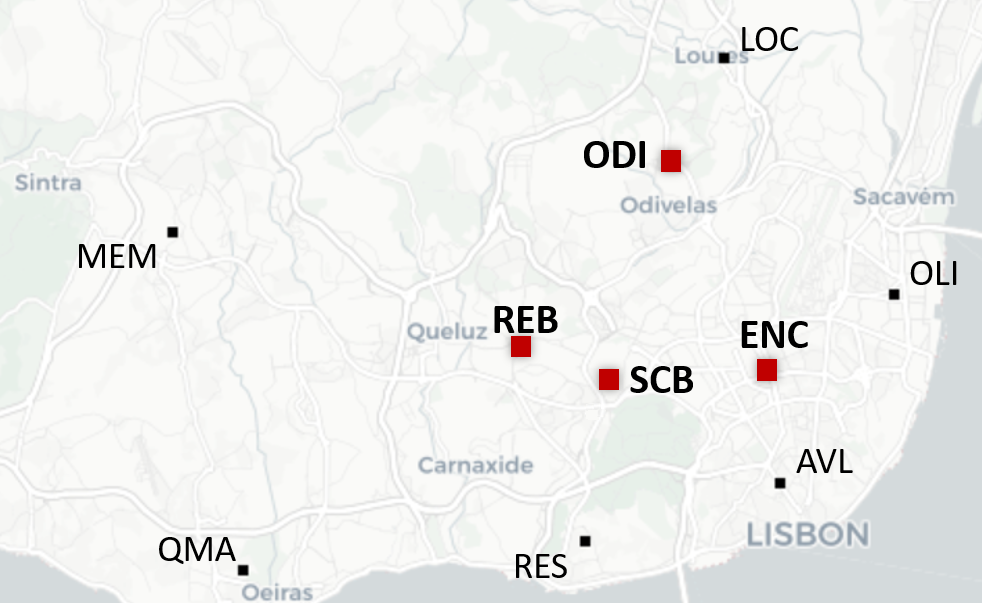
\includegraphics[width=0.7\textwidth]{./Images/map-filtered.png}
\caption{Stations in the greater area of Lisbon used in this work.}
\label{fig:map-filtered}
\end{figure}

\subsection{Spatial interpolation Algorithms Implementation}

In order to assess algorithm performance, cross validation tests were applied to the selected stations. In each iteration, one measure from one central station (\Cref{fig:map-filtered}) was inferred using the measures from remaining stations in the same time interval. In \Cref{main-pseudocode} the pseudo-code of the setup of this process is presented.

\begin{center}
\begin{algorithm}[H]
\linespread{1.35}\selectfont
\SetAlgoLined
 dataset = extractDataset()\;
 stations = stationsData()\;
 centralStations = centralStationsData()\;
 \ForEach{set in dataset}{
  \ForEach{station in stations}{
   \If{station in centralStations}{
    executeInterpolationAlgorithms(station, set)\;
   }
  }
 }
 \caption{Pseudo-code of the algorithm execution setup.}
 \label{main-pseudocode}
\end{algorithm}
\end{center}

Both LI and NN were implemented with the python \textit{scipy} library \textit{interpolate} package.

In what regards IDW, its only user defined parameter is the power function value \textit{p}, which defines how the weight of each observed point varies with the distance to the estimated point. This algorithm was implemented in Python.
Cross validation was applied to decide which is the best value of \textit{p} for the selected data.

OK is the Kriging variant which was considered in this work, and it was implemented with the \textit{pykrige} python library \cite{PyKrige2019}.

Variograms can only be modelled if datasets have a relative high number of points and spatial density, which is not the case in this work, in which observation points are only 10 and sparsely distributed \cite{Mesquita2009}.
Cross validation was applied to decide which is the best Kriging variogram for this work selected data.

\subsection{FBN Implementation}

FBNs have several implementation details which are user defined.

\begin{itemize}[leftmargin=0.0mm]
  \item[] \textbf{Antecedent and Consequent Areas}
\end{itemize}

\noindent
First, the amount of antecedent and consequent areas that constitute the network, and which variables are associated to each area, must be defined. The dataset PM10 values and its coordinates are the variables used. The interpolation objective is to model a value for the PM concentration at a specific location, with a respective pair of coordinates. Therefore, there are two independent variables, represented as antecedent areas - latitude and longitude - and one unknown value, represented as consequent area - PM10 concentration.

\begin{itemize}[leftmargin=0.0mm]
  \item[] \textbf{Variables Scale Conversion}
\end{itemize}

\noindent
Since each area only receives inputs between 0 and 1, the values of all used variables (latitude, longitude and PM10 concentration) need to be converted to the same scale, and a maximum value needs to be defined, to represent 100\% ratio of its corresponding area.

In the case of the coordinates, delimiting values were represented by the outline of the most exterior stations. 

The station at the extreme west location is \ac{MEM} whose longitude is -9.347222, and the extreme east station is \ac{OLI} with a longitude of -9.108056. Therefore, the longitude defined value for 0 is -9.35 and for 1 is -9.1.

The same was done for the latitude. The southest station is \ac{QMA}, which has latitude equal to 38.6975, and the northest is \ac{LOC} whose latitude is 38.829722. Therefore, the defined values for 0 and 1 for the antecedent area corresponding to the latitude coordinate are 38.69 and 38.83 respectively.

With these settings it is possible to define the spatial grid presented in \Cref{fig:scale-converted-grid}.

\begin{figure}[ht]
\centering
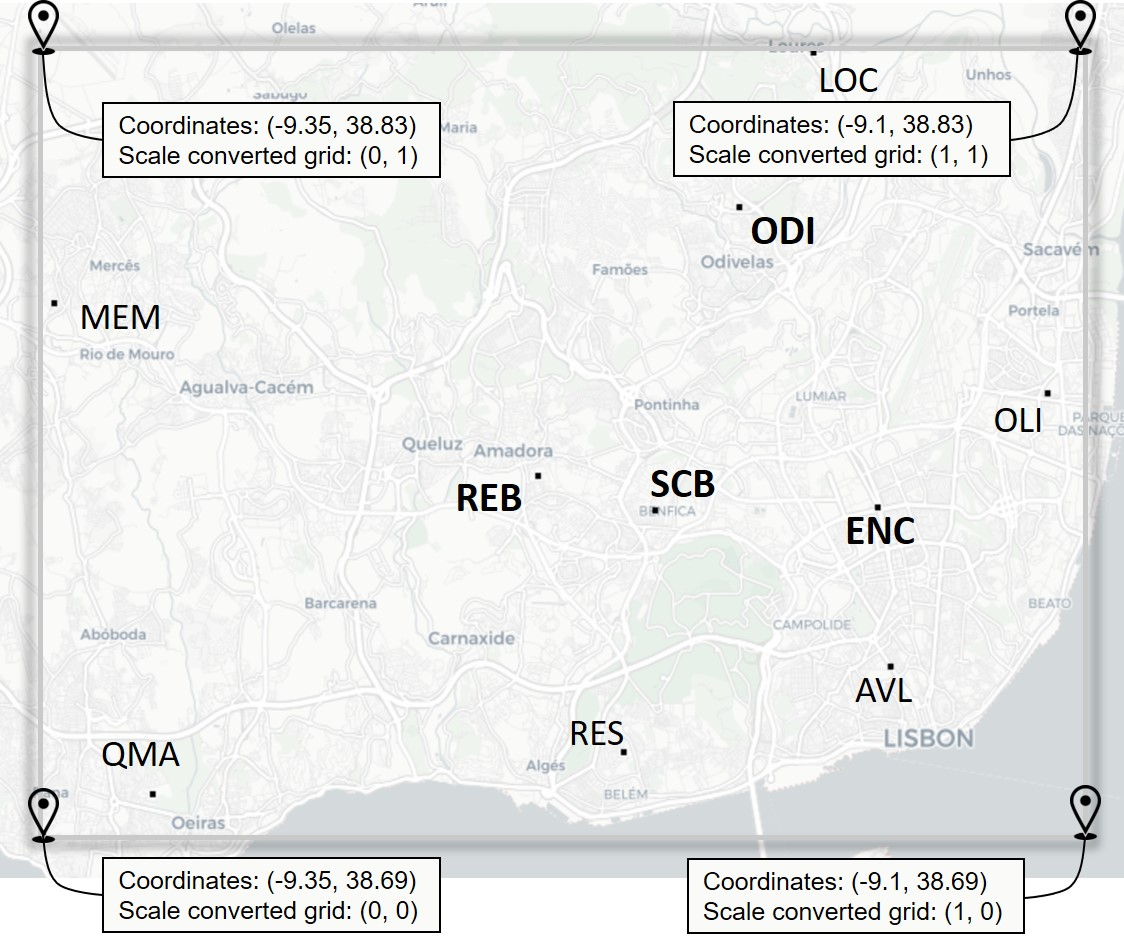
\includegraphics[width=0.8\textwidth]{./Images/scale-converted-grid.jpg}
\caption{Spatial grid used for FBN coordinate scale conversion.}
\label{fig:scale-converted-grid}
\end{figure}

Finally, for the PM10 concentration values, the minimum value was 0 μg/m³ and the maximum value was 175 μg/m³, which is above the highest registered value in the filtered 5 year dataset.

The equations from \Cref{longitude} to \Cref{pm10-concentration} represent the scale transformations used for each variables, longitude, latitude and PM10 concentration.

\begin{equation} 
\label{longitude}
\scalebox{1.4}{$ Lon_{val} = \dfrac{Lon_{station}-Lon_{min}}{Lon_{max}-Lon_{min}} $}
\end{equation}

\begin{equation} 
\label{latitude}
\scalebox{1.4}{$Lat_{val} = \dfrac{Lat_{station}-Lat_{min}}{Lat_{max}-Lat_{min}}$}
\end{equation}

\begin{equation} 
\label{pm10-concentration}
\scalebox{1.4}{$PM10_{val} = \dfrac{PM_{observed}}{175}$}
\end{equation}

%As already noted, the ALV station was excluded from the dataset due to its farther location compared to every other station. Both its longitude and latitude coordinates would represent extreme values to the scale transformation which could be detrimental to FBN execution, since it would decrease the data spatial density, namely the latitude maximum value would increase significantly the respective axis scale.

\begin{itemize}[leftmargin=0.0mm]
  \item[] \textbf{Parametrization}
\end{itemize}

\noindent
In order to better explain and understand FBN performance in this work application, several parametrizations were tested.
The user defined parameters which were tested are the number of antecedent and consequent areas in the network, the number of testing and training epochs, the granularity and the number of samples.

Training and testing epochs were tested on how its increase, independently of the network size, influences results. Furthermore, net size along with number of samples and granularity were also tested to conclude how these parameters can provide a better accuracy against time of execution through cross validation in the selected dataset.

In order to analyse how resolution of data influences FBNs interpolation performance results, these were tested with a dataset of 15 minutes intervals values measured at monitoring stations. This dataset was provided by CCDR-LVT, and contained only measures from the stations AVL, ENC, OLI, RES and SCB.

Additionally, FBNs were tested with data from four 15 minute sets of values per hour, to infer an average for that hour at the location of each station. This was different than previous tests, in which only hourly averages were used to train and were infered by FBNs.

%OK, IDW and FBNs were executed with the hourly average sets for the corresponding period, as a control measure of increases in performance between FBN executions. Afterwards, FBNs were solely trained with the 15 minutes intervals. The only difference between both FBN implementations, is the number of training sets. In the implementation which received only hour averages as inputs, there was only one set of training sets for each interpolation. In the implementation with 15 minutes measures, there were 4 training sets.


\begin{itemize}[leftmargin=0.0mm]
  \item[] \textbf{Implementation}
\end{itemize}

\noindent
The implementation of FBN was the result of previous works \cite{Tome2014}. This implementation was migrated from Python 2 to Python 3, and code was additionally developed to insert every training and testing rule in the networks directly from an excel dataset. This enables the interpolation of several datasets in only one execution.

%One of the goals of this work is to experiment and compare \ac{FBN}s performance against state-of-the-art algorithms for the spatial interpolation of air pollution, namely \ac{PM10} and \ac{PM2.5}, such as Kriging and \ac{ANN} based models. For this its better parameters need to be defined. This will be made through the use of the cross validation technique further explained in the following section.

%FBN functioning was already explained in section XX, therefore it is known that for its implementation several parameters need to be previously assessed and defined in order to get the best results possible with the lowest amount of execution time.
%These parameters are the number of samples, …
%Several tests with the data explained above will be made in this study in order to define the best parameters for this problem.

%In the original implementation of FBNs, several files need to be previously written with the details of the details, specifications and user defined parameters of the FBN.

%the rules of the learning and the training process which consist of…

%and the data for the inference process which consists of…

%In order to systemize this, a python program was developed to write these files automatically without the need to write these files.
%This program reads the training data directly from the excel provided by APA in the case of the hourly data, or the excel filled by the pre mentioned python program with the quarter of an hour data, the user can define the fbn parameters directly in the code, and the program further produces the files needed for the FBN execution.
%The 15 to 15 data provided by the CCDR-LVT were presented in a normal text file with no specific format. A python program was made to export these to excel, for them to be used by the above systematic program.

\subsection{Algorithm Performance Evaluation}

In order to assess the results of the cross validation approach, the statistical error parameters presented in equations \eqref{mae} and \eqref{rmse} were considered.

\begin{equation} 
\label{mae}
\scalebox{1.4}{ $ MAE = \dfrac{\sum_{i=1}^{n} |M_i - O_i|}{n}$}
\end{equation}

\begin{equation} 
\label{rmse}
\scalebox{1.4}{ $ RMSE = \sqrt[2]{\dfrac{1}{n}\sum_{i=1}^{n} {(M_i - O_i)}^{2}}$}
\end{equation}

%\begin{equation} 
%\label{r2}
%\scalebox{1.4}{ $ {R}^{2} = 1 - \dfrac{\sum_{i=1}^{n} {(O_i %- M_i)}^{2}}{\sum_{i=1}^{n} {(O_i - \overline{O_i})}^{2}}$}
%\end{equation}

Where $M_i$ represents the modelled value, $O_i$ represents the observed value and $n$ is the total of inferences.% and $\overline{O_i}$ is the mean of the observed values.

\ac{MAE} measures the average magnitude of errors in a set of predictions. \ac{RMSE} is a quadratic parameter which also measures the average magnitude of the error.
Both express average model prediction error in units of the variable of interest, which for PM10 concentration are μg/m³. Regarding RMSE, since errors are squared before they are averaged, increased weight is given to large errors.

%${\textrm{R}}^{2}$ is a statistical measure that represents the proportion of the variance of a dependent variable that is explained by the independent variables. 

%According to directive 2008/50/EC, the measure of the uncertainty

%max uncertainty is 25\%.
%uncertainty = (observed value - modelled value)/ limit value
%averaging period one day: 50 μg/m3
%calendar year: 40

%\begin{equation} 
%\label{uncertainty}
%\scalebox{1.3}{$ uncertainty = \dfrac{O - M}{limit\: value} $}
%\end{equation}

%Where $M$ is the modelled value, 

% #############################################################################
\section{System for Online Data Visualization} 

The system for online data visualization is composed of a database, an html, css and javascript apache website with a javascript library which provides custom map web visualization and rendering, Mapbox GL JS.

\subsection{Database}

A MongoDB database was developed to store the values obtained by monitoring systems. Depending on the performance of the developed low-cost system, several of its replicas could be placed around Lisbon, in locations where there are no other monitoring stations, in order to complement and increase the density of data for the city of Lisbon.

MongoDB was the database technology chosen for this specific application, due to its high scalability and flexibity. It is a NoSQL type of database, which stores data in flexible, JSON-like documents. It is a distributed database at its core, therefore it has high availability through built-in replication, and horizontal scalability with native sharding, with end-to-end security. Each database contains collections, which in turn contain documents. Documents are filled with fields and the size and content of documents in the same collection can vary.

The database used in this work only has one collection, in which every measure from the system is saved. Despite the non-enforcement of document structure in the database, for the purpose of this work, each valid document must have date, location, sensor ID and pm10 value as valid fields, and the date field along with the sensor ID can not be repeated in different documents.

\subsection{Mapbox GL JS}

Mapbox is a provider of custom online maps for websites and applications. The company was founded in 2010 and has contributed to, and created, several tools which let developers use custom maps in their own platforms. It has emerged as a response to the limited choice offered by map providers such as Google Maps. Some of these tools are open source mapping libraries and applications, such as the Mapbox GL JS JavaScript library, the MBTiles specification, the TileMill cartography IDE, the Leaflet JavaScript library and the CartoCSS map styling language and parser \cite{Mapbox2019}.

Mapbox GL JS is a JavaScript library which uses WebGL to render interactive maps from vector tiles and Mapbox styles, and it was used in this work to represent the results of the real-time spatial interpolation PM10 values.

Its online map implementations are widely customizable and allow the visualization of a wide variety of data representations in the chosen map, such as polygons, icons, buildings, polygons, 3D models and animations.

In this work, extrusion of polygons was used to represent the levels of estimated PM10 concentration values, whose height and color is determined by the pollution value in each point of the map.

For the representation of these polygons, a grid was defined, which is delimited by the coordinates of the Lisbon monitoring station networks which are on the edges of the city. This is a convex hull grid, with a resolution of 100 m². For these extrusions to be included, a geojson file was created, with the polygons of every element in the defined grid. A python script is running in the background which updates the values at each station every hour, performs a new interpolation with the updated values, and updates the geojson file accordingly.

Regarding the javascript implementation, a Map object, which represents the whole map visualization, is defined in the main website file. In the javascript code of the webpage, the geojson file, which should be saved in a local directory, is accessed, and then its respective extrusions are inserted in the Map object, which is rendered when users access the webpage.

%\subsection{API}

% Ideally there should be an API - Ou então dizer que é apenas um servidor Apache
% The part about the python script needs to be changed once this change is % done.

% #############################################################################